\documentclass{beamer}
\usepackage[utf8]{inputenc}
\usepackage[frenchb]{babel}
\usepackage{color}

\title{Détection de collisions}
\subtitle{Géométrie algorithmique - INFO-F-420}
\author{Tim Lenertz}
\institute{ULB, MA1 INFO}
\date{\today}

\usetheme{Antibes}
\usecolortheme{whale}

\begin{document}

\begin{frame}
	\titlepage
\end{frame}

\begin{frame}
	\tableofcontents
\end{frame}

\section{Introduction}

\begin{frame}{Introduction}
	\begin{itemize}
	\item Espace 2D/3D avec objets géométriques animés
	\item Détecter collisions de façon dynamique
	\item Ex. simulations physiques, jeux video, robotique, ...
	\item Temps réel $\rightarrow$ Algorithmes efficaces
	\item Calcul d'intersection, distance entre objets
	\item Structure de données des objets
	\item Subdivision de l'espace
	\end{itemize}
\end{frame}

\begin{frame}{A posteriori}
	\begin{itemize}
	\item Faire avancer simulation
	\item Intersection de produit
	\item $\rightarrow$ Corriger, traitement de collision
	\item ex. appliques lois cinétiques
	\end{itemize}
\end{frame}

\begin{frame}{A priori}
	\begin{itemize}
	\item Prédire collisions
	\item Intersection ne se produisent jamais
	\item Calcul de temps/point d'inpact futur
	\item ex. controlleur système réel
	\end{itemize}
\end{frame}

\subsection{Bounding boxes}

\begin{frame}{Bounding boxes}
	\begin{itemize}
	\item Enveloppe simple autour d'objet
	\item ex. rectangle, sphère, polygone convexe
	\item Permet exclure collision en $O(1)$
	\end{itemize}
	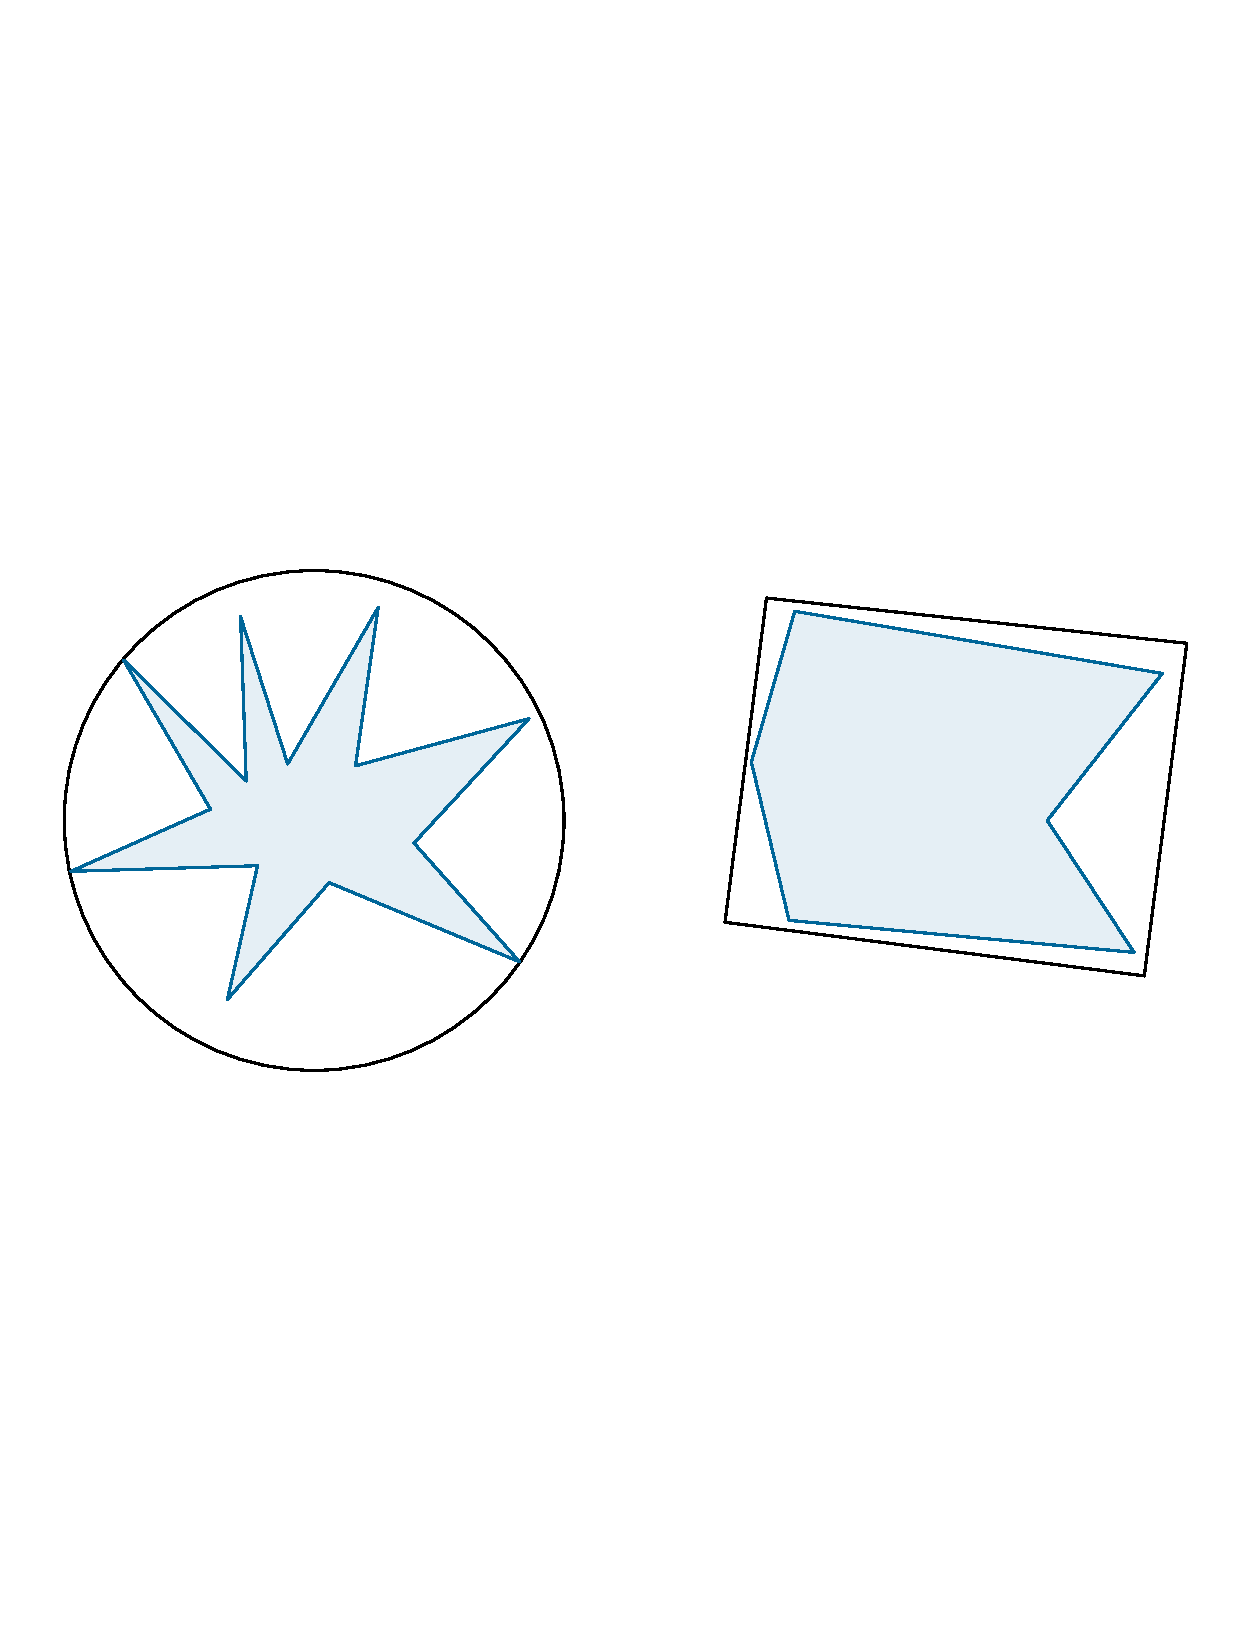
\includegraphics[width=8cm]{bounding.png}
\end{frame}

\subsection{Subdivision d'espace}

\begin{frame}{Subdivision d'espace}
	\begin{itemize}
	\item Scène complexe avec bcp d'objets
	\item Peu de collisions possibles ($\ll n^{2}$)
	\item Regrouper objets proches / collisions potentielles
	\item Exclure majorité des tests
	\end{itemize}
\end{frame}

\begin{frame}{Grille uniforme}
	\begin{columns}[c]
	\begin{column}[T]{.5\textwidth}
		\begin{itemize}
		\item Cellules carrées/cubiques de ême taille
		\item Enregistrer objets/cellule
		\item Tester seulement ds même cellule
		\item Bonne performance si objets distribués uniformement
		\end{itemize}
	\end{column}
	\begin{column}[T]{.5\textwidth}
		\includegraphics[width=5cm]{unigrid.png}
	\end{column}
	\end{columns}
\end{frame}

\begin{frame}{Grille uniforme (2)}
	\begin{columns}[c]
	\begin{column}[T]{.5\textwidth}
		\begin{itemize}
		\item Clustering
		\item Cellules trop grandes/petites
		\item Dégénère vers $O(n^2)$
		\end{itemize}
	\end{column}
	\begin{column}[T]{.5\textwidth}
		\includegraphics[width=5cm]{unigrid2.png}
	\end{column}
	\end{columns}
\end{frame}


\begin{frame}{Bounding Volume Hierarchy}
	\begin{itemize}
	\item Regrouper objets dans arbre (dynamique)
	\item Tester d'abord \emph{bounding boxes} des groupements
	\item Peut atteindre $O(\log n)$
	\end{itemize}
	\begin{center}
	\includegraphics[width=4cm]{bvh.png}
	\end{center}
\end{frame}


\begin{frame}{Autres optimisations}
	\begin{itemize}
	\item Quadtree/Octree
	\item Binary Space Partition
	\item View Frustum Culling
	\item ...
	\end{itemize}
\end{frame}

\subsection{Polygones convexes}
\begin{frame}{Introduction}
	\begin{itemize}
	\item Traité ici: polygones convexes (2D)
	\item Algorithmes: intersection, distance minimale
	\item en $O(\log n)$
	\end{itemize}
\end{frame}

\section{Intersection droite-polygone convexe}
\subsection{Fonction unimodale}

\begin{frame}{Fonction unimodale}
	\begin{itemize}
	\item Fonction réelle sur entiers $f : \{ 1, 2, ..., n \} \rightarrow \mathbb{R}$
	\item Existe entire $m \in [1, n]$
	\item $f$ strictement $\nearrow$ ($\searrow$) en $[1, m]$ et str. $\searrow$ ($\nearrow$) en $[m+1, n]$
	\item Exemple:
	\end{itemize}
	\begin{center}
	\includegraphics[width=4cm]{unimodal.png}
	\\
	$m = 6$
	\end{center}
\end{frame}

\begin{frame}{Trouver maximum et minimum}
	\begin{itemize}
	\item Comparer $f(1)$ et $f(2)$, pour déterminer si $\nearrow\searrow$ ou $\searrow\nearrow$
	\item $\nearrow\searrow$: Minimum = $\min \{ f(1), f(n) \}$, Maximum = $m$
	\item $\searrow\nearrow$: Maximum = $\max \{ f(1), f(n) \}$, Minimum = $m$
	\item Recherche dichotomique: Trouver point où signe de $f(i+1) - f(i)$ change
	\item Complexité logarithmique $O(\log n)$
	\end{itemize}
	\begin{center}
	\includegraphics[width=4cm]{unimodal.png}
	\\
	$m = 6$
	\end{center}
\end{frame}

\subsection{Fonction bimodale}

\begin{frame}{Fonction bimodale}
	\begin{itemize}
	\item Décalage circulaire d'une fonction unimodale
	\item Il existe $r \in [1,n]$ tel que $f(r),f(r+1),...,f(n),f(1),f(2),...,f(r-1)$ est unimodale
	\item Deux extréma à l'intérieur
	\item Soit $\nearrow\searrow\nearrow$ et $f(1) > f(n)$, ou $\searrow\nearrow\searrow$ et $f(1) < f(n)$
	\end{itemize}
	\begin{center}
	\includegraphics[width=4cm]{bimodal.png}
	\\
	$\min = f(2); \max = f(8)$
	\end{center}
\end{frame}

\begin{frame}{Trouver maximum et minimum}
	\begin{itemize}
	\item Pour le cas $f(1) < f(n)$ et $\searrow\nearrow\searrow$:
	\item Si $f(2) < (1)$:
		\begin{itemize}
		\item Soit $T(x)$ droite de $(1, f(1))$ à $(n, f(n))$ ($\nearrow$){}
		\item Soit $g(x) = \min \{ T(x), f(x) \}$
		\item $g$ est unimodale, $\min f$ = $\min g$
		\item $\max f$ dans séq. unimodale $f(m+1),f(m+2),...,f(n)$
		\item Donc on trouve min et max en $O(\log n)$
		\end{itemize}
	\item Si $f(2) > f(1)$: $f(1)$ est minimum, maximum est dans $f(2)...f(n)$ (unimodal)
	\end{itemize}
	\begin{center}
	\includegraphics[width=4cm]{unibi.png}
	\\
	$f$ en vert, $g$ en vert+bleu
	\end{center}
\end{frame}

\subsection{Bimodalité sur polygone convexe}

\begin{frame}{Distances orientées}
	\begin{columns}[c]
	\begin{column}[T]{.5\textwidth}
		\begin{itemize}
		\item Soit $P$ polygone convexe
		\item $\{ p_{1}, p_{2}, ..., p_{n} \}$ points en sens horlogique
		\item $d(p_{i}, L)$ = distance orthogonale de $p_{i}$ à $L$
		\item Distance orientée $h(p_{i}, L, v)$:
			\begin{itemize}
			\item $= d(p_{i}, L)$ si $p_{i}$ et $v$ sur même côté de $P$
			\item $= -d(p_{i})$ sinon
			\end{itemize}
		\item $h(i) = h(p_{i}, L, v)$ bimodale
		\end{itemize}
	\end{column}
	\begin{column}[T]{.5\textwidth}
		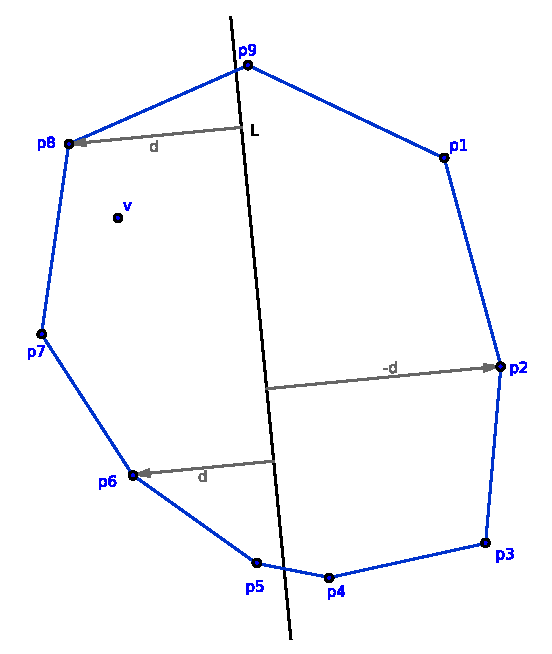
\includegraphics[width=5cm]{h.eps}
	\end{column}
	\end{columns}
\end{frame}


\begin{frame}{Démonstration bimodalité de $h$}
	\begin{columns}[c]
	\begin{column}[T]{.6\textwidth}
		\begin{itemize}
		\item Soit $p_{k}$ point qui minimise $h$
		\item Montrer que $f(k), f(k+1), ..., f(k-1)$ est unimodale (indices modulo $n$):
			\begin{itemize}
			\item $r$ vecteur directeur de $L$ (avec $\angle(r, p_{i}p_{i+1}) < \pi$)
			\item $h(i+1) = h(i) + |p_{i}p_{i+1}| \sin a_{i}$
			\item $a_{i+1} = a_{i} - b_{i+1}$
			\item $b_{i} < \pi$ car $P$ est convexe
			\item $\sum b_{i} = 2\pi$
			\item $\sin a_{k}, \sin a_{k+1}, ... \sin_{k-1}$ positive, puis négative
			\item Donc $f(k), f(k+1), ..., f(k-1)$ unimodale $\Box$
			\end{itemize}
		\end{itemize}
	\end{column}
	\begin{column}[T]{.4\textwidth}
		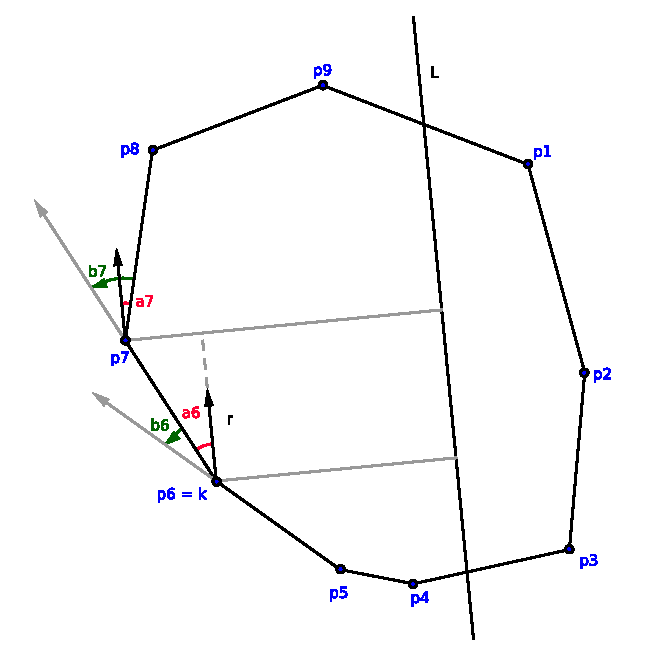
\includegraphics[width=5cm]{hBimodal.eps}
	\end{column}
	\end{columns}
\end{frame}


\subsection{Algorithme IGL}

\begin{frame}{Algorithme IGL}
	\begin{columns}[c]
	\begin{column}[T]{.5\textwidth}
		\begin{itemize}
		\item Trouver points $P \cap L$ en temps logarithmique
		\item Utiliser $h(p_{i}, L, p_{1})$ bimodale
		\item Soit $p_{k}$ minimum de $h$
		\item Si $h(k) > 0$:
			\begin{itemize}
			\item Tous les points sur même côté de $P$
			\item (= côté de $p_{1}$)
			\item donc pas d'intersection
			\end{itemize}
		\item Si $h(k) = 0$:
			\begin{itemize}
			\item $p_{k}$ est unique point d'intersection
			\item Autres points tous sur même côté
			\end{itemize}
		\end{itemize}
	\end{column}
	\begin{column}[T]{.5\textwidth}
		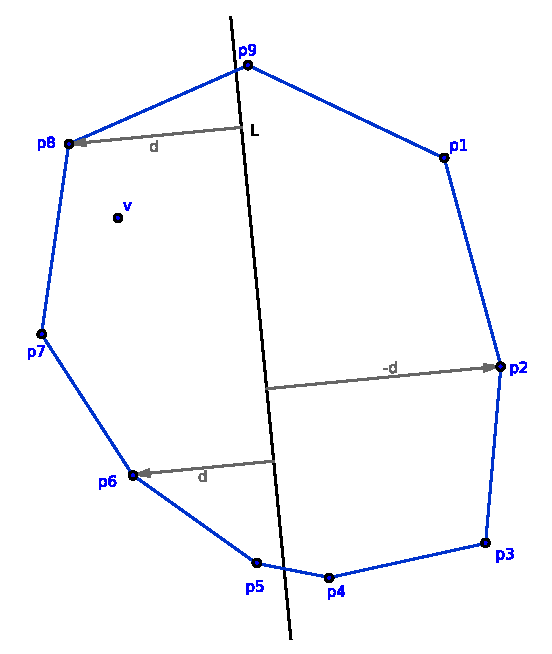
\includegraphics[width=5cm]{h.eps}
	\end{column}
	\end{columns}
\end{frame}

\begin{frame}{Algorithme IGL (2)}
	\begin{columns}[c]
	\begin{column}[T]{.5\textwidth}
		\begin{itemize}
		\item Si $h(k) < 0$:
			\begin{itemize}
			\item 2 points d'intersection
			\item Sur segments $p_{i}p_{i+1}$\\
				pour lesquels\\
				$h(i) \times h(i+1) < 0$
			\item Recherche dichotomique sur séq. monotones\\
				$h(k),h(k+1),...,h(n)$ et\\
				$h(1),h(2),...,h(k)$
			\item ($p_{1}$ côté opposé de $p_{k})$
			\item Calculer $p_{i}p_{i+1} \cap L$
			\end{itemize}
		\item Donc points d'intersection trouvés en $O(\log n)$ $\Box$
		\end{itemize}
	\end{column}
	\begin{column}[T]{.5\textwidth}
		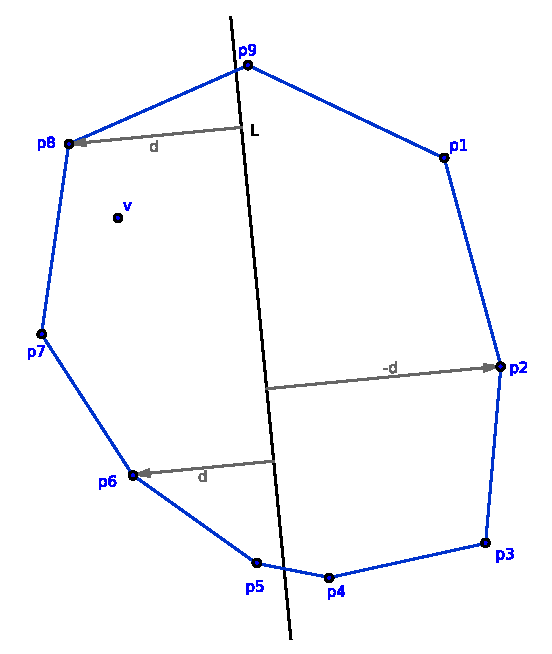
\includegraphics[width=5cm]{h.eps}
	\end{column}
	\end{columns}
\end{frame}

\begin{frame}
	\Large{Démo}
\end{frame}


\section{Intersection de deux polygones convexes}
\subsection{Généralisations}

\begin{frame}{Généralisations}
	\begin{itemize}
	\item Généralisation de l'algo précédent
	\item Sur objets convexes 2D et 3D
	\item Temps logarithmiques
	\item On intersecte l'intérieur des objets
	\item Complexités:
		\begin{description}
		\item[droite-droite] $O(1)$
		\item[droite-polygone] $O(\log n)$
		\item[droite-plan] $O(1)$
		\item[droite-polyhédron] $O(\log^{2} n)$
		\item[polygone-polygone] $O(\log n)$
		\item[polygone-plan] $O(\log n)$
		\item[polygone-polyhédron] $O(\log^{2} n)$
		\item[plan-plan] $O(1)$
		\item[plan-polyhédron] $O(\log^{2} n)$
		\item[polyhédron-polyhédron] $O(\log^{3} n)$
		\end{description}
	\end{itemize}
\end{frame}

\subsection{Algorithme IGG}

\begin{frame}{Algorithme IGG}
	\begin{columns}[c]
	\begin{column}[T]{.5\textwidth}
		\begin{itemize}
		\item Reduire à intersection de deux polylignes
		\item Elimination binaire
		\item $O(\log (n + m))$
		\end{itemize}
	\end{column}
	\begin{column}[T]{.5\textwidth}
		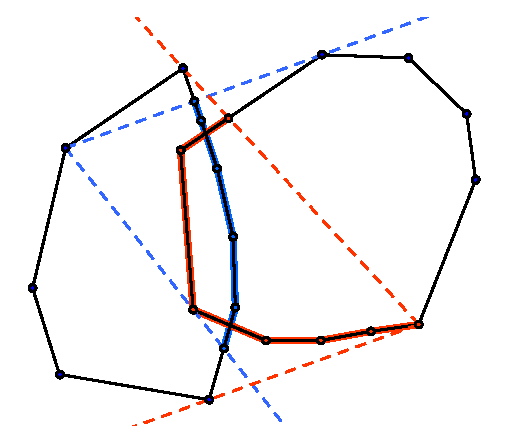
\includegraphics[width=5cm]{igg1.eps}
	\end{column}
	\end{columns}
\end{frame}

\begin{frame}{Phase initiale (1)}
	\includegraphics[width=10cm]{igg2.pdf}
	\begin{itemize}
	\item $q \in Q$ quelconque
	\item $a, b = p_{1}q \cap Q$ (algorithme IGL)
	\item Si $p_{1} \in ab$, intersection en $p_{1}$
	\end{itemize}
\end{frame}

\begin{frame}{Phase initiale (2)}
	\includegraphics[height=5cm]{igg3.pdf}
	\begin{itemize}
	\item Déduire polylignes $L_{v}$ et $L_{w}$
	\item Intersections $C_{1} \cap Q$ + points de $Q$ (même pour $P$)
	\item Possible en $O(\log n)$ par IGL
	\item $P$ et $Q$ intersectent ssi $L_{v}$ et $L_{w}$ intersectent 
	\end{itemize}
\end{frame}

\begin{frame}
	\Large{Démo}
\end{frame}

\begin{frame}{Phase itérative}
	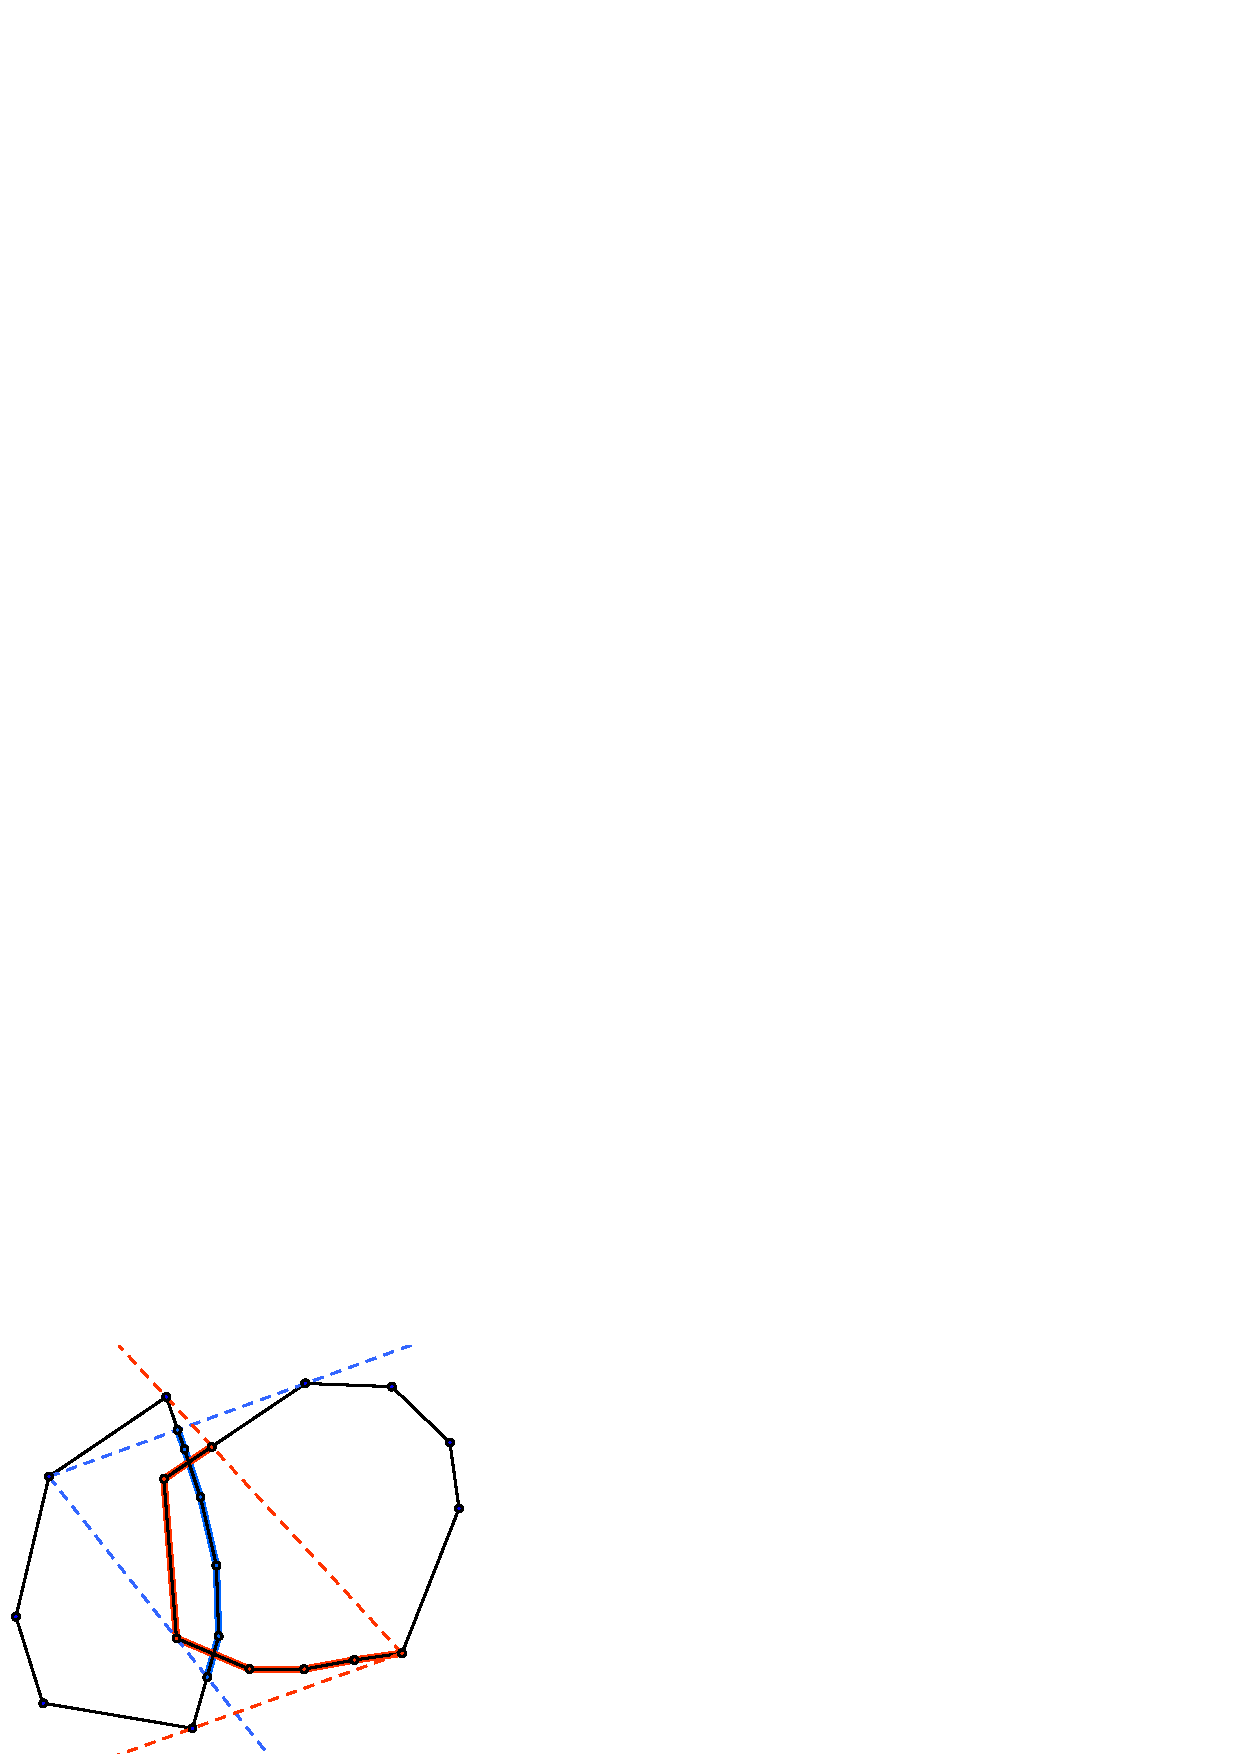
\includegraphics[height=3cm]{igg1.jpg}
	\begin{itemize}
	\item Soit $n = |L_{v}|$, $m = |L_{w}|$
	\item Tant que $n, m > 5$ (sinon, différent algorithme)
	\item $i = \lfloor \frac{n}{2} \rfloor$ et $j = \lfloor \frac{m}{2} \rfloor$
	\item $F, G = v_{i}v_{i+1} \cap AYBX$ (avec $v_{i+1} \in v_{i}F$)
	\item $E, H = w_{j}v_{j+1} \cap AYBX$ (avec $w_{j+1} \in v_{j}H$)
	\item Eliminer à chaque étape moitié de $L_v$ et/ou $L_w$
	\end{itemize}
\end{frame}

\begin{frame}
	\Large{Détail algorithme}
\end{frame}

\section{Distance minimale de deux polygones convexes}

\begin{frame}{Distance minimale de deux polygones convexes}
	\begin{itemize}
	\item Segment $d$ de longueur minimale qui relie $P$ et $Q$
	\item Détection collisions \emph{à priori}
	\item Algorithme en $O(\log n + \log m)$
	\item 3 cas possibles: point-point, point-droite, droite-droite
	\item droite-droite: parallèles, = point-droite
	\end{itemize}
	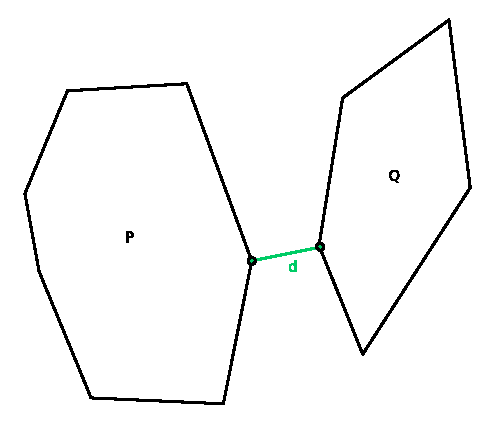
\includegraphics[width=3cm]{dpp.eps} \hspace{0.5cm}
	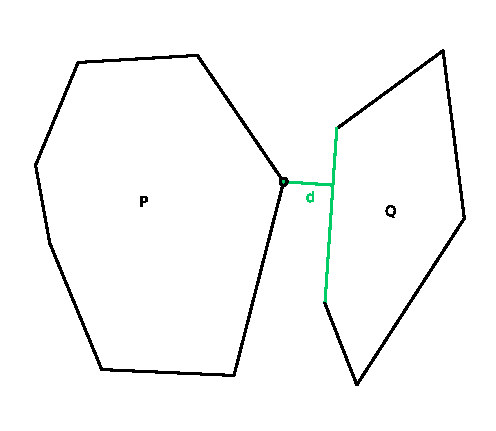
\includegraphics[width=3cm]{dpl.eps} \hspace{0.5cm}
	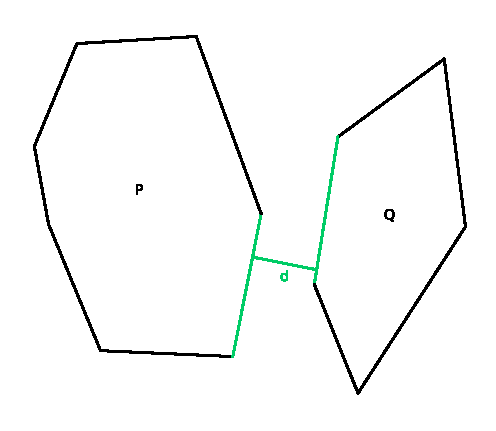
\includegraphics[width=3cm]{dll.eps}
\end{frame}


\begin{frame}{Preuve 3 cas possibles}
	\begin{columns}[c]
	\begin{column}[T]{.5\textwidth}
		\begin{itemize}
		\item Soit $d = pq$
		\item $p, q$ doivent être sur bord des polygones
		\item $p$ et/ou $q$ doit être coin de polygone 
		\item Eliminer cas où $p$ \textbf{et} $q$ sont sur segments:
			\begin{itemize}
			\item Soit $p \in e_{p}$ et $q \in a_{q}$
			\item Alors $e_{p} \parallel e_{q}$
			\item $\exists$ projection orthogonale de point de \\$e_{p}$ ($e_{q}$) sur $e_{q}$ ($e_{p}$)
			\end{itemize} 
			$\Box$
		\end{itemize}
	\end{column}
	\begin{column}[T]{.5\textwidth}
		\includegraphics[width=5cm]{dmincases.png}
	\end{column}
	\end{columns}
\end{frame}

\subsection{Algorithme d'élimination binaire}

\begin{frame}{Phase initiale}
	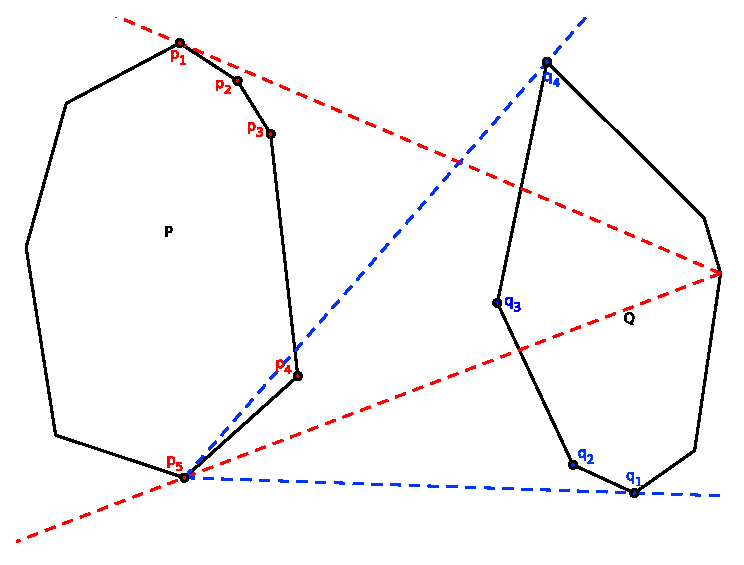
\includegraphics[height=5.5cm]{dmininit1.eps}
	\begin{itemize}
	\item Déterminer $C_{1}$ et $C_{2}$
	\item Polylignes $L_{p}$ et $L_{q}$ dans $P$ et $Q$
	\item $d$ doit relier $L_{p}$ et $L_{q}$
	\end{itemize}
\end{frame}

\begin{frame}{Phase itérative}
	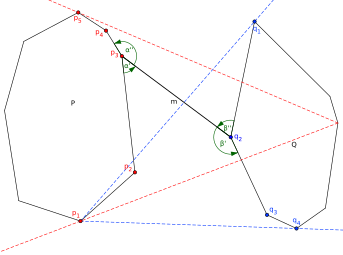
\includegraphics[height=5cm]{dmin.eps}
	\begin{itemize}
	\item $i = \lfloor \frac{n}{2} \rfloor$ et $j = \lfloor \frac{m}{2} \rfloor$, $m = p_{i}q_{j}$
	\item $\alpha' + \alpha'' \geq \pi$ et donc $\alpha' \geq \frac{\pi}{2}$ ou $\alpha'' \geq \frac{\pi}{2}$
	\item $\alpha' + \beta' \leq \pi$ implique $\alpha' < \beta''${}
	\item $\alpha' + \beta' > \pi$ ou $\alpha'' + \beta'' > \pi$
	\end{itemize}
\end{frame}

\begin{frame}{Phase itérative (2)}
	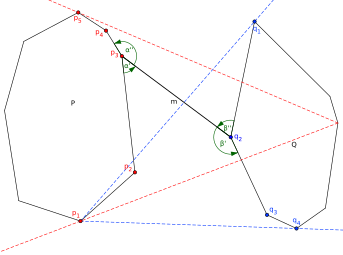
\includegraphics[height=5cm]{dmin.eps}
	\begin{itemize}
	\item Eliminer moitié de $L_p$ et/ou $L_q$
	\item Jusqu'à $|L_p|, |L_p| \leq 2$
	\item Distinguer cas selon $|L_p|$ et $|L_p|$
	\end{itemize}
\end{frame}

\begin{frame}{Cas 1: $|L_p| = 1$}
	\begin{columns}[c]
	\begin{column}[T]{.5\textwidth}
		\begin{itemize}
		\item Si $\beta' \geq \frac{\pi}{2}$: $q_{\text{first}} \leftarrow q_{j}$
		\item Si $\beta'' \geq \frac{\pi}{2}$: $q_{\text{last}} \leftarrow q_{j}$
		\item $|L_q| = 1$ est symétrique
		\item Au moins une condition doit être vraie
		\item $\leftarrow$ On élimine tjs moitié
		\end{itemize}
	\end{column}
	\begin{column}[T]{.5\textwidth}
		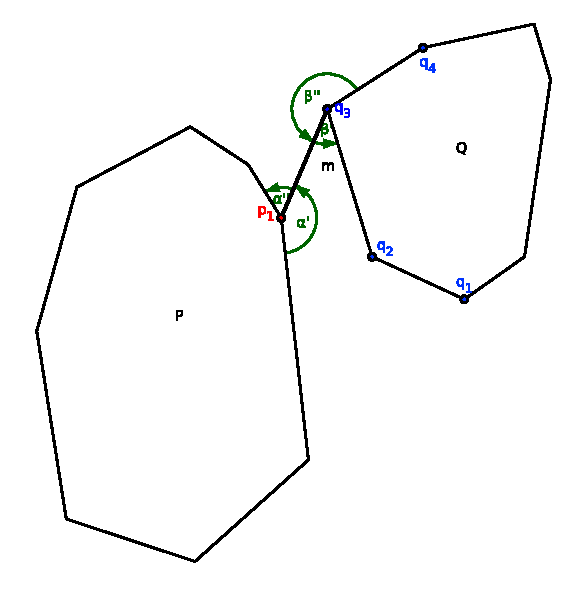
\includegraphics[width=5cm]{dmin1.eps}
	\end{column}
	\end{columns}
\end{frame}

\begin{frame}{Cas 2: $|L_p| = 2$}
	\begin{columns}[c]
	\begin{column}[T]{.5\textwidth}
		Si $m$ sort de $P$:
		\begin{enumerate}
		\item Si $\alpha' + \beta' > \pi$:\\
			\hspace{0.3cm} \textcolor{gray}{Si $\alpha' \geq \frac{\pi}{2}$, $p_{\text{first}} \leftarrow p_{2}$}\\
			\hspace{0.3cm} \textcolor{gray}{Si $\beta' \geq \frac{\pi}{2}$, $q_{\text{first}} \leftarrow q_{j}$}
		\item \textcolor{blue}{Si $\beta'' \geq \frac{\pi}{2}$: $q_{\text{last}} \leftarrow q_{j}$}
		\item ...
		\end{enumerate}
	\end{column}
	\begin{column}[T]{.5\textwidth}
		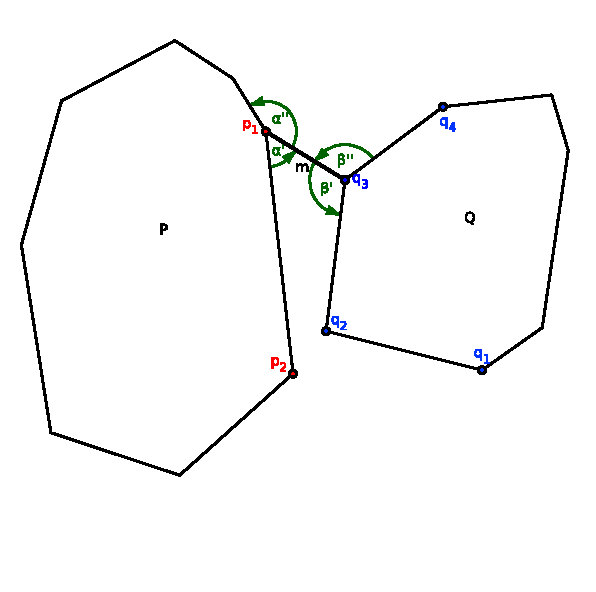
\includegraphics[width=5cm]{dmin2_1.eps}
	\end{column}
	\end{columns}
\end{frame}

\begin{frame}{Cas 2: $|L_p| = 2$}
	\begin{columns}[c]
	\begin{column}[T]{.5\textwidth}
		Si $m$ sort de $P$:
		\begin{enumerate}
		\item Si \textcolor{blue}{$\alpha' + \beta' > \pi$}: \\
			\hspace{0.3cm} Si $\alpha' \geq \frac{\pi}{2}$, $p_{\text{first}} \leftarrow p_{2}$\\
			\hspace{0.3cm} \textcolor{blue}{Si $\beta' \geq \frac{\pi}{2}$, $q_{\text{first}} \leftarrow q_{j}$}
		\item \textcolor{blue}{Si $\beta'' \geq \frac{\pi}{2}$: $q_{\text{last}} \leftarrow q_{j}$}
		\item ...
		\end{enumerate}
	\end{column}
	\begin{column}[T]{.5\textwidth}
		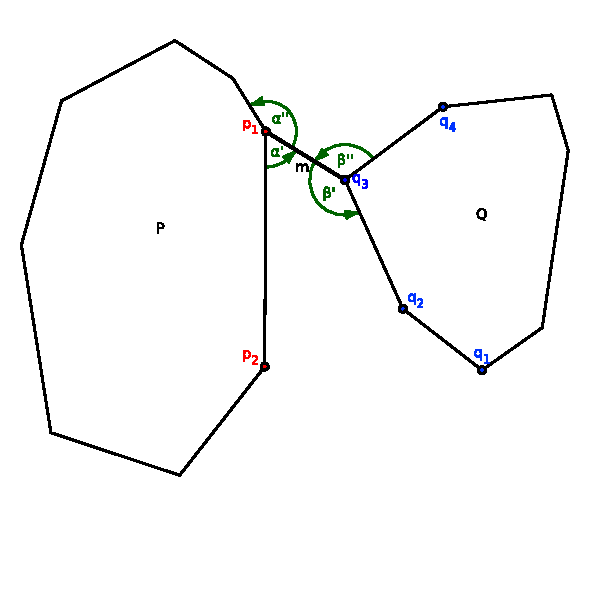
\includegraphics[width=5cm]{dmin2_2.eps}
	\end{column}
	\end{columns}
\end{frame}

\begin{frame}{Cas 2: $|L_p| = 2$}
	\begin{columns}[c]
	\begin{column}[T]{.5\textwidth}
		Si $m$ sort de $P$:
		\begin{enumerate}
		\item Si $\alpha' + \beta' > \pi$: \\
			\hspace{0.3cm} \textcolor{gray}{Si $\alpha' \geq \frac{\pi}{2}$, $p_{\text{first}} \leftarrow p_{2}$}\\
			\hspace{0.3cm} \textcolor{gray}{Si $\beta' \geq \frac{\pi}{2}$, $q_{\text{first}} \leftarrow q_{j}$}
		\item \textcolor{blue}{Si $\beta'' \geq \frac{\pi}{2}$: $q_{\text{last}} \leftarrow q_{j}$}
		\item ...
		\end{enumerate}
	\end{column}
	\begin{column}[T]{.5\textwidth}
		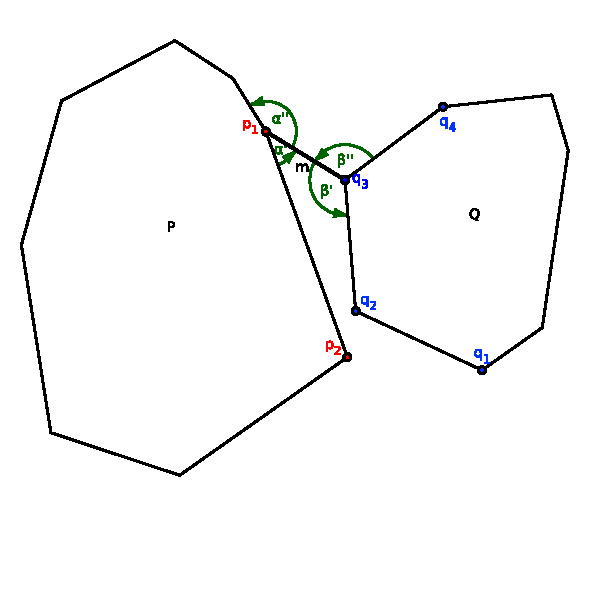
\includegraphics[width=5cm]{dmin2_3.eps}
	\end{column}
	\end{columns}
\end{frame}

\begin{frame}{Cas 2: $|L_p| = 2$}
	\begin{columns}[c]
	\begin{column}[T]{.5\textwidth}
		Si $m$ sort de $P$:
		\begin{enumerate}
		\item Si \textcolor{blue}{$\alpha' + \beta' > \pi$}: \\
			\hspace{0.3cm} Si $\alpha' \geq \frac{\pi}{2}$, $p_{\text{first}} \leftarrow p_{2}$\\
			\hspace{0.3cm} \textcolor{blue}{Si $\beta' \geq \frac{\pi}{2}$, $q_{\text{first}} \leftarrow q_{j}$}
		\item Si $\beta'' \geq \frac{\pi}{2}$: $q_{\text{last}} \leftarrow q_{j}$
		\item ...
		\end{enumerate}
	\end{column}
	\begin{column}[T]{.5\textwidth}
		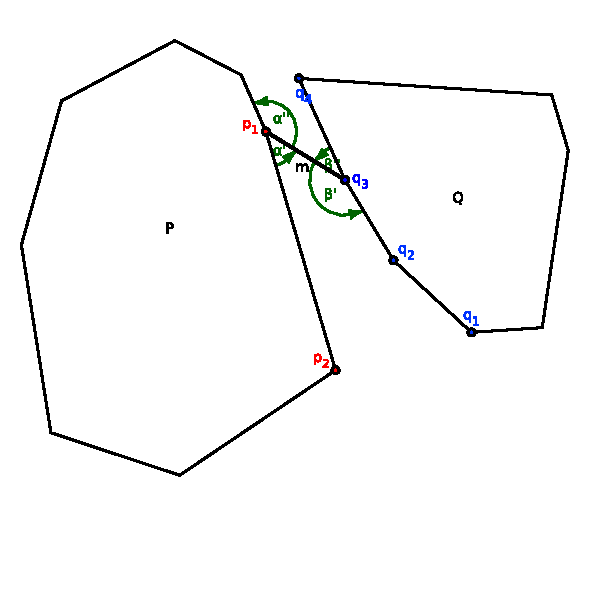
\includegraphics[width=5cm]{dmin2_4.eps}
	\end{column}
	\end{columns}
\end{frame}

\begin{frame}{Cas 2: $|L_p| = 2$ (2)}
	\begin{columns}[c]
	\begin{column}[T]{.5\textwidth}
		Si $m$ sort de $P$:
		\begin{enumerate}
		\item Si \textcolor{blue}{$\alpha' + \beta' > \pi$}: \\
			\hspace{0.3cm} Si $\alpha' \geq \frac{\pi}{2}$, $p_{\text{first}} \leftarrow p_{2}$\\
			\hspace{0.3cm} \textcolor{blue}{Si $\beta' \geq \frac{\pi}{2}$, $q_{\text{first}} \leftarrow q_{j}$}
		\item \textcolor{blue}{Si $\beta'' \geq \frac{\pi}{2}$: $q_{\text{last}} \leftarrow q_{j}$} \\ 
			\hspace{0.5cm} \vdots
		\item Si \textcolor{blue}{$\alpha' < \beta'' < \frac{\pi}{2}$}:
			\begin{itemize}
			\item \textcolor{blue}{Si proj orth $q_{j}$ sur $p_{1}p_{2}$ existe: $q_{\text{last}} \leftarrow q_{j}$}
			\item Sinon: $p_{\text{last}} \leftarrow p_{\text{1}}$
			\end{itemize}
		\end{enumerate}
	\end{column}
	\begin{column}[T]{.5\textwidth}
		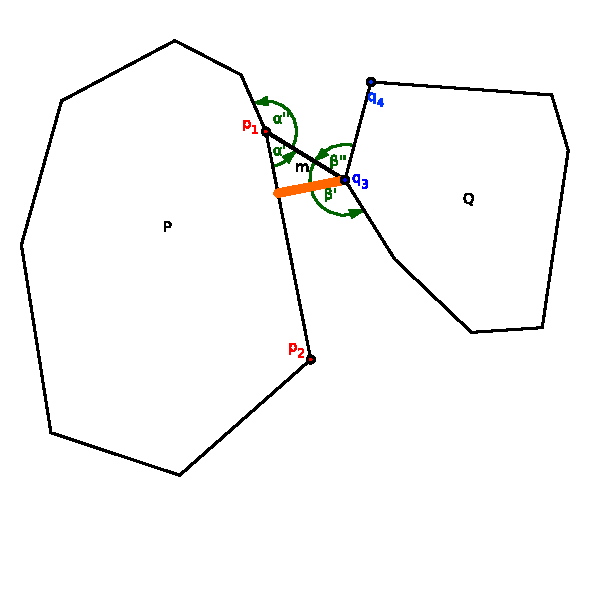
\includegraphics[width=5cm]{dmin2_5.eps}
	\end{column}
	\end{columns}
\end{frame}


\begin{frame}{Cas 2: $|L_p| = 2$ (2)}
	\begin{columns}[c]
	\begin{column}[T]{.5\textwidth}
		Si $m$ sort de $P$:
		\begin{enumerate}
		\item Si \textcolor{blue}{$\alpha' + \beta' > \pi$}: \\
			\hspace{0.3cm} Si $\alpha' \geq \frac{\pi}{2}$, $p_{\text{first}} \leftarrow p_{2}$\\
			\hspace{0.3cm} \textcolor{blue}{Si $\beta' \geq \frac{\pi}{2}$, $q_{\text{first}} \leftarrow q_{j}$}
		\item Si $\beta'' \geq \frac{\pi}{2}$: $q_{\text{last}} \leftarrow q_{j}$ \\ 
			\hspace{0.5cm} \vdots
		\item Si \textcolor{blue}{$\alpha' < \beta'' < \frac{\pi}{2}$}:
			\begin{itemize}
			\item Si proj orth $q_{j}$ sur $p_{1}p_{2}$ existe: $q_{\text{last}} \leftarrow q_{j}$
			\item \textcolor{blue}{Sinon: $p_{\text{last}} \leftarrow p_{\text{1}}$}
			\end{itemize}
		\end{enumerate}
	\end{column}
	\begin{column}[T]{.5\textwidth}
		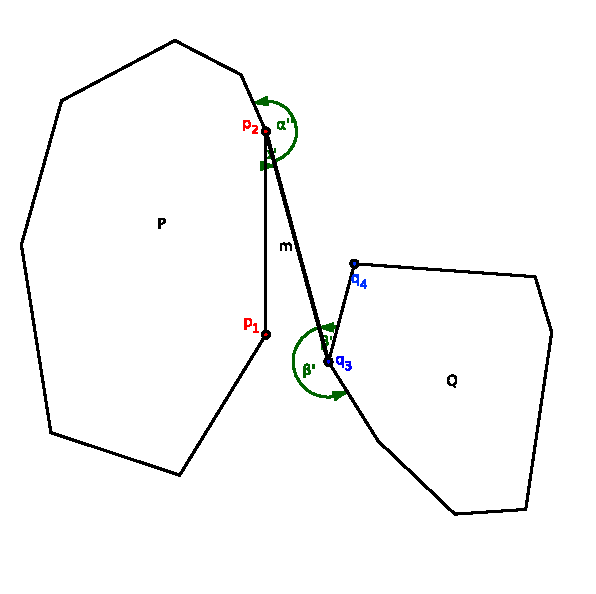
\includegraphics[width=5cm]{dmin2_6.eps}
	\end{column}
	\end{columns}
\end{frame}

\begin{frame}{Cas 2: $|L_p| = 2$ (2)}
	\begin{columns}[c]
	\begin{column}[T]{.5\textwidth}
		Si $m$ sort de $P$:
		\begin{enumerate}
		\item Si \textcolor{blue}{$\alpha' + \beta' > \pi$}: \\
			\hspace{0.3cm} Si $\alpha' \geq \frac{\pi}{2}$, $p_{\text{first}} \leftarrow p_{2}$\\
			\hspace{0.3cm} \textcolor{blue}{Si $\beta' \geq \frac{\pi}{2}$, $q_{\text{first}} \leftarrow q_{j}$}
		\item Si $\beta'' \geq \frac{\pi}{2}$: $q_{\text{last}} \leftarrow q_{j}$ \\ 
			\hspace{0.5cm} \vdots
		\item Si $\alpha' < \beta'' < \frac{\pi}{2}$:
			\begin{itemize}
			\item \textcolor{gray}{Si proj orth $q_{j}$ sur $p_{1}p_{2}$ existe: $q_{\text{last}} \leftarrow q_{j}$}
			\item \textcolor{gray}{Sinon: $p_{\text{last}} \leftarrow p_{\text{1}}$}
			\end{itemize}
		\end{enumerate}
	\end{column}
	\begin{column}[T]{.5\textwidth}
		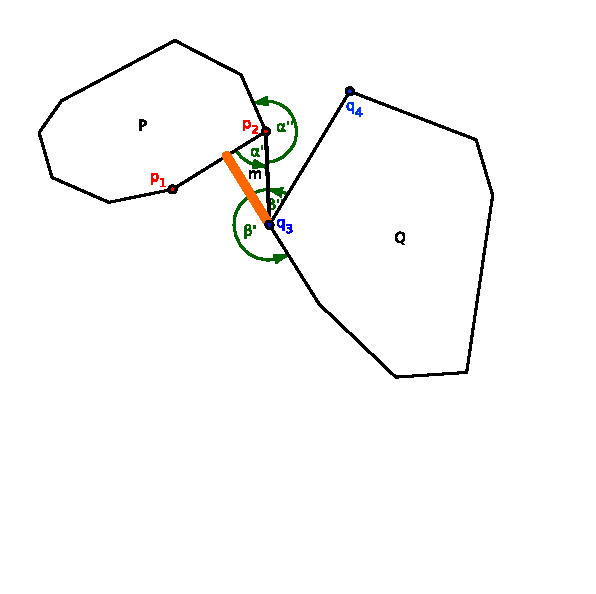
\includegraphics[width=5cm]{dmin2_7.eps}
	\end{column}
	\end{columns}
\end{frame}


\begin{frame}{Cas 2: $|L_p| = 2$ (3)}
	\begin{columns}[c]
	\begin{column}[T]{.5\textwidth}
		Si $m$ entre dans $P$:
		\begin{itemize}
		\item $p_{\text{last}} \leftarrow p_{1}$
		\item Si $\beta' \geq \pi$: $q_{\text{first}} \leftarrow q_{j}$
		\item \textcolor{blue}{Si $\beta'' \geq \pi$: $q_{\text{last}} \leftarrow q_{j}$}
		\end{itemize}
	\end{column}
	\begin{column}[T]{.5\textwidth}
		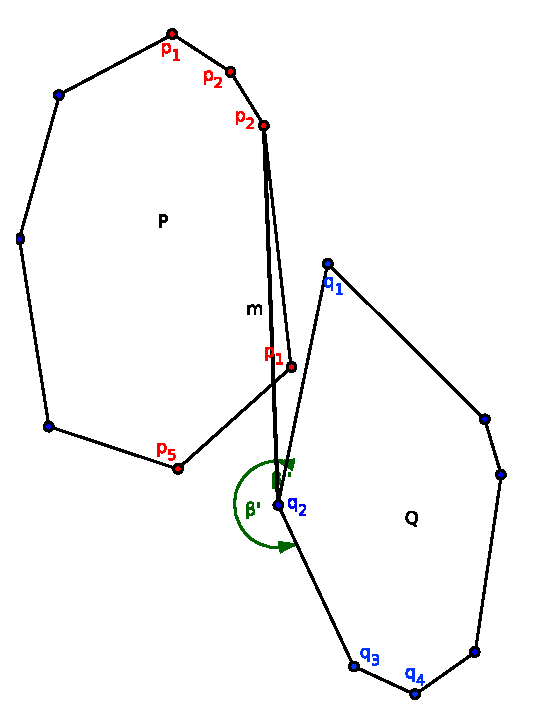
\includegraphics[width=5cm]{dmin2_8.eps}
	\end{column}
	\end{columns}
\end{frame}


\begin{frame}{Cas 3: $|L_p| \geq 3$ et $|L_q| \geq 3$}
	\begin{columns}[c]
	\begin{column}[T]{.5\textwidth}
		Si $m$ sort de $P$ et de $Q$:
		\begin{enumerate}
		\item \textcolor{blue}{Si $\alpha' + \beta' > \pi$}:\\
			\hspace{0.3cm} Si $\alpha' \geq \frac{\pi}{2}$: $p_{\text{first}} \leftarrow p_{i}$ \\
			\hspace{0.3cm} \textcolor{blue}{Si $\beta' \geq \frac{\pi}{2}$: $q_{\text{first}} \leftarrow q_{j}$}
		\item Si $\alpha'' + \beta'' > \pi$:\\
			\hspace{0.3cm} \textcolor{gray}{Si $\alpha'' \geq \frac{\pi}{2}$: $p_{\text{last}} \leftarrow p_{i}$} \\
			\hspace{0.3cm} \textcolor{gray}{Si $\beta'' \geq \frac{\pi}{2}$: $q_{\text{last}} \leftarrow q_{j}$}
		\end{enumerate}
		Si $m$ entre dans $P$ ou $Q$: \\
			\hspace{0.3cm} similaire au cas précédent
	\end{column}
	\begin{column}[T]{.5\textwidth}
		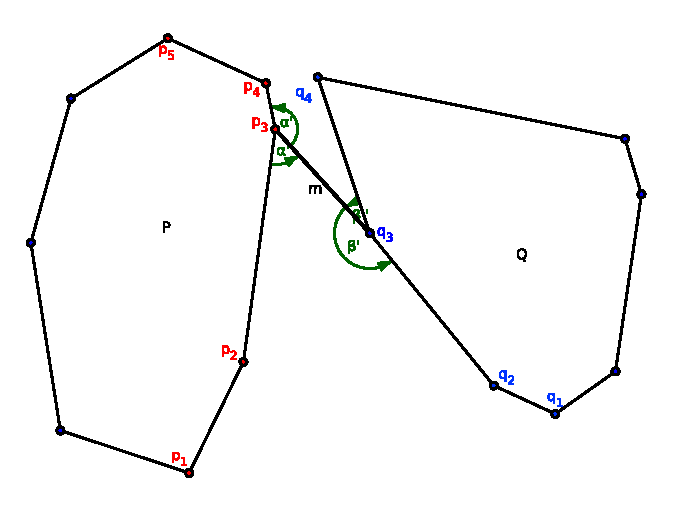
\includegraphics[width=5cm]{dmin3_1.eps}
	\end{column}
	\end{columns}	
\end{frame}

\end{document}
